\documentclass[a4paper, 12pt]{article}
% for linebreaks and sectioning commands in german
\usepackage[ngerman]{babel}
% Encoding for German sonderzeichen
\usepackage[utf8]{inputenc}
% for size of borders etc.
\usepackage{geometry}
% for hyperlinks
\usepackage[hidelinks]{hyperref}
% for some nice pics
\usepackage{graphicx}
% for algorithm env
\usepackage{algpseudocode, algorithm}
% for math env
\usepackage{mathtools}
% for Color in Equations
\usepackage[usenames,dvipsnames]{xcolor}
% for caption of pics????
\usepackage{caption}
% for caption of subfigures???
\usepackage{subcaption}
% for listing some code in a language
\usepackage{listings}

% for listingsenv
\definecolor{mygreen}{rgb}{0,0.6,0}
\definecolor{mygray}{rgb}{0.5,0.5,0.5}
\definecolor{mymauve}{rgb}{0.58,0,0.82}
\lstset{ %
  backgroundcolor=\color{white},   % choose the background color; you must add \usepackage{color} or \usepackage{xcolor}
  basicstyle=\scriptsize,        % the size of the fonts that are used for the code
  breakatwhitespace=false,         % sets if automatic breaks should only happen at whitespace
  commentstyle=\color{mygreen},    % comment style
  keepspaces=true,                 % keeps spaces in text, useful for keeping indentation of code (possibly needs columns=flexible)
  keywordstyle=\color{blue},       % keyword style
  %morekeywords={*,...,isfield,/,+,-},            % if you want to add more keywords to the set
  numbers=left,                    % where to put the line-numbers; possible values are (none, left, right)
  numbersep=5pt,                   % how far the line-numbers are from the code
  numberstyle=\tiny\color{gray}, % the style that is used for the line-numbers
  rulecolor=\color{black},         % if not set, the frame-color may be changed on line-breaks within not-black text (e.g. comments (green here))
  stringstyle=\color{BurntOrange}, % string literal style
  showstringspaces=false,          % underline spaces within strings only
  tabsize=2,                       % sets default tabsize to 2 spaces
  title=\lstname                   % show the filename of files included with \lstinputlisting; also try caption instead of title
}
% set size env
\geometry{a4paper,left=25mm,right=25mm, top=2cm, bottom=2cm}



\begin{document}

% Title Page
\input{./title_page_1.tex}

% Table of Contents
\pagenumbering{roman}
\tableofcontents
\newpage
\pagenumbering{arabic}


% Fragestellungen Insgesamt:
% - Was sind die wesentlichen Parameter der Anwendung?
% - Welche Parameter der Anwendung sind schon beim Entwurf bekannt?
% - Was muss eingestellt werden?
% - Wo wird ein lernfähiges System benötigt?
% - Welche prinzipiellen Problemstellungen sind in einem solchen LFS gegeben?
% - Welche Anforderungen bestehen an so ein System?
% - Welche Eigenschaften ändern sich zur Betriebszeit?
% - Wie wird darauf reagiert?
% - Welche Probleme können auftreten?
% - Wie kann das Auftreten von Problemen festgestellt werden?
% - Welche Aspekte sind anwendungsspezifisch?
% - Welche Aspekte sind allgemeingültig?

% Fragestellungen für die Literaturarbeit:
% - Kategorisierung des Lernverfahrens:
% - 1. / 2. Ordnung?
% - Größen a, b, c, d, zur Beschreibung?
% - Designparameter?
% - Robustheit gegenüber ...
% - Rauschen?
% - Ausreißern?
% - Umgang mit Zeitvarianz?
% - Annahmen und Voraussetzungen, insbesondere implizite Annahmen?
% - Welche Performancemaße werden verwendet?
% - Designaufwand, Rechenaufwand und Speicherbedarf?
% - Grenzen der Verfahren?
% - Vorteile und Nachteile im Vergleich zu anderen Verfahren?

% - Was muss eingestellt werden?
% - Welche Probleme können auftreten?
% - Wie kann das Auftreten von Problemen festgestellt werden?
% - Welche Aspekte sind anwendungsspezifisch?
% - Welche Aspekte sind allgemeingültig?
% - Designaufwand, Rechenaufwand und Speicherbedarf?
% - Grenzen der Verfahren?
% - Vorteile und Nachteile im Vergleich zu anderen Verfahren?

\section{Einleitung}
\label{sec:einleitung}
Wenn die Eingangssignale eines adaptiven Filters mit Impulsen versetzt sind kann dies zu einem verzerrten Adaptionsverhalten führen. Hierbei stellen Impulse bzw. Ausreißer Datenpunkte dar, welche nicht in den Lernprozess miteinbezogen werden sollen. Die Entstehung solcher Impulse variiert je nach Anwendung. Beispielsweise können die Daten durch eine Signalübertragung beschädigt worden sein und daher Werte aufweisen, welche das Lernverhalten verfälschen können.

Ein Lernverfahren, welches mit impulsversetzten Daten umgehen kann, ist das adaptive Filter \emph{Recursive Least M-estimate (RLM)} \cite{zou2000recursive}. Ziel dieser Ausarbeitung ist das Vorstellen und Bewerten dieses Verfahrens.

Zu Beginn wird in Abschnitt (\ref{sec:rlm}) der RLM vorgestellt. In Abschnitt (\ref{sec:performance}) wird auf die Performance des RLM in verschiedenen Szenarien eingegangen und jeweils bewertet. Zum Schluss wird in Abschnitt (\ref{sec:zusammenfassung}) diese Ausarbeitung zusammengefasst.


\section{Recursive Least M-Estimate (RLM)}
\label{sec:rlm}
Zunächst wird in Abschnitt (\ref{sec:rlm:einleitung}) eine Einführung in die Arbeitsprozesse robuster Lernverfahren gegeben. Anschließend wird das Lernverfahren des RLM erläutert. Dazu wird zunächst kurz die Funktionsweise des \emph{Recursive Least Squares (RLS)} Algorithmus beschrieben (Abschnitt (\ref{sec:rlm:rls})), da dieser die Grundlage des RLM darstellt. Anschließend wird auf die Unterschiede beider Lernverfahren eingegangen und die Funktionsweise des RLM im Detail beschrieben (Abschnitt (\ref{sec:rlm:rlm})).

\subsection{Robuste Lernverfahren}
\label{sec:rlm:einleitung}
\begin{figure}[H]
    \centering
    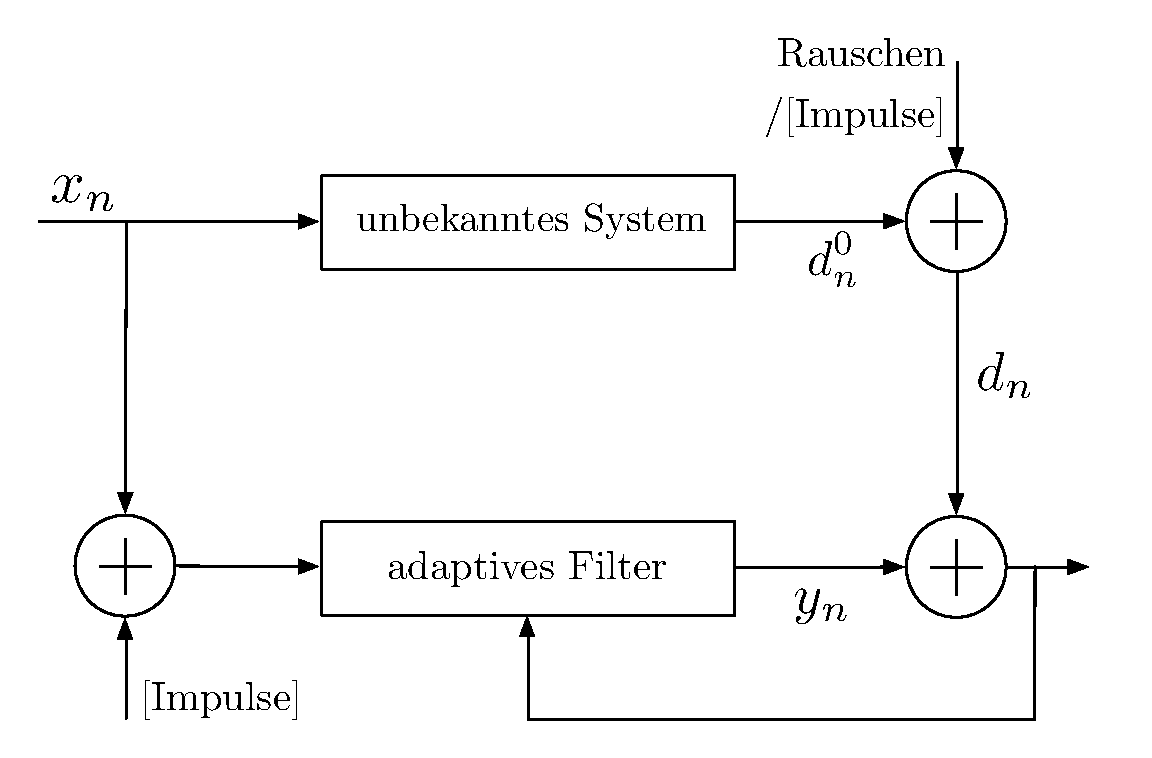
\includegraphics[width=0.6\textwidth]{./images/system_identification.eps}
    \caption{Struktur eines Lernprozesses (Vergleiche Quelle: \cite{zou2000recursive}).}
    \label{fig:struktur_lernprozess}
\end{figure}
In Abb. (\ref{fig:struktur_lernprozess}) ist die Struktur des Lernprozesses eines robusten adaptiven Filters zu sehen. Ziel des Lernverfahrens ist die Annäherung seines Outputs an den des unbekannten Systems (US). Das US steht für die abstrakte Betrachtung der Zielfunktion, die approximiert werden soll. Sei $x_n$ das Lerndatum zum Zeitpunkt $n$, welches den Input des adaptiven Filters darstellt, so soll der Output des Filters $y_n$ möglichst nah am Output des US $d^0_n$ liegen.
Als Herausforderung stellt sich heraus, dass das Datum welches dem Lernverfahren für den Vergleich zur Verfügung steht mit Rauschen versetzt sein kann. Folglich findet die Annäherung von $y_n$ an $d_n = Rauschen+d^0_n$ statt. Als $Rauschen$ wird im Rahmen dieser Ausarbeitung eine Gaussverteilte Zufallsvariable angenommen.
Nachdem das Filter seinen Output $y_n$ generiert hat wird der Fehler $e_n$ zu $d_n$ berechnet und es werden die Parameter des Filters in Abhängigkeit von $e_n$ angepasst.

Eine weitere Herausforderung sind impulsversetzte Daten. Dabei kann $x_n$ oder $d_n$ mit Impulsen versetzt sein. Ein Impuls lässt sich als Offset betrachten, welches auf die entsprechenden Werte addiert wird.
Robuste Lernverfahren haben als Aufgabe diese Impulse zu erkennen und ihre Wirkung auf die Adaption zu hemmen. 

Im dieser Ausarbeitung wird sich implizit auf impulsversetzte $d_n^0$-Werte bezogen, da die Implementation der Impulse in Matlab so durchgeführt wurde.

\subsection{RLS}
\label{sec:rlm:rls}
Der \emph{Recursive Least Squares (RLS)} Algorithmus \cite[p.~195ff]{diniz1997adaptive} ist ein Lernverfahren 2. Ordnung, welches den quadratischen Fehler auf allen gegebenen Daten minimiert.
In den Gleichungen (\ref{eq:rlm:rls:alpha}) und (\ref{eq:rlm:rls:s}) sind allgemeine Formeln für Lernverfahren 2. Ordnung zum Update von $\alpha_n$ und $S_n$ zu sehen.
\begin{align}
    \label{eq:rlm:rls:alpha}
	\alpha_n &= a \cdot \alpha_{n-1} + b\cdot(y_n-\tilde{y}_n)) \cdot S_{n-1} \varphi(x_n)\\
    \label{eq:rlm:rls:s}
	S_{n} &= c \cdot S_{n-1} + d \cdot S_{n-1} \varphi(x_n) \varphi(x_n)^T S_{n-1}
\end{align}
$\alpha_n$ stellt den Parametervektor und $S_n$ die Korrelationsmatrix des Lernverfahrens dar. $y_n$ ist der gewünschte und $\tilde{y}_n$ der berechnete Output. Es gilt $\tilde{y}_n = \alpha_n \varphi(x_n)$ wobei $\varphi(x_n)$ die Anwendung des Inputs $x_n$ auf die verwendeten Basisfunktionen ausdrückt.

Die Festlegung der Koeffizienten $a, b, c, d$ identifiziert ein solches Lernverfahren eindeutig. 
Im Falle des RLS sind die Belegungen der Koeffizienten in den Gleichungen (\ref{eq:rlm:rls:ac}) und (\ref{eq:rlm:rls:bd}) zu sehen.
\begin{align}
    \label{eq:rlm:rls:ac}
	a &= c=1\\
    \label{eq:rlm:rls:bd}
	b&=d=\frac{1}{\lambda+\varphi(x_n)^T S_{n-1} \varphi(x_n)}
\end{align}
$0 \ll \lambda<1$ wird auch als \emph{Vergessenheitsfaktor} bezeichnet. Aufgrund seines antiproportionalen Einflusses in $b$ und $d$ trägt ein hoher Wert zu einer stärkeren Vernachlässigung neuer Werte auf die Änderung von $\alpha_n$ und $S_n$ bei.



\subsection{RLM}
\label{sec:rlm:rlm}
Der \emph{Recursive Least M-estimate} (\emph{RLM}) Algorithmus \cite{zou2000recursive} ist ein robuster Lernalgorithmus, welcher auf Basis des RLS arbeitet.
Es soll zunächst grob auf die mathematische Herleitung des Algorithmus eingegangen werden bevor im Anschluss die Eigenschaften des RLM diskutiert werden.

\vspace{5mm}
Die Loss-Funktion des RLM ist gegeben als:
\begin{equation*}
    \label{eq:rlm:rlm:l}
    L_n=\sum_{i = 0}^{n}\lambda^{n-i}\rho(e_i)
\end{equation*}
Hierbei sei $e_n$ definiert als der aktuelle Fehler $e_n = y_n - \tilde{y}_n$.
Die abschnittweise definierte Funktion $\rho(e_n)$ 
\begin{equation*} 
\rho(e)=\begin{cases}
    \label{eq:rlm:rlm:p}
      \frac{e^2}{2} & 0 < |e| < \xi, \\
      \xi |e| - \frac{\xi^2}{2} & \xi \leq |e| < \Delta_1, \\
      \frac{\xi^2}{2}(\Delta_2 + \Delta_1) - \frac{\xi^2}{2} + \frac{\xi}{2} \frac{(|e|-\Delta_2)^2}{\Delta_1-\Delta_2}& \Delta_1 \leq |e| < \Delta_2, \\
      \frac{\xi}{2}(\Delta_2+\Delta_1) - \frac{\xi^2}{2} & \Delta_2 \leq |e|
   \end{cases}
\end{equation*}
stellt den \emph{M-Estimate}, bzw. \emph{M-Schätzer} dar und bildet vom aktuellen Fehler $e_n$ auf einen positiven reellen Wert ab. Auf die Eigenschaften von $\rho(e_n)$, insbesondere ihre Grenzen $\xi$, $\Delta_1$ und $\Delta_2$, wird später eingegangen.
Die Wahl der Loss-Funktion $L_n$ ist ein entscheidender Punkt in der Unterscheidung mit anderen Lernverfahren. Beispielsweise verwendet der RLS als Loss-Funktion den quadrierten aktuellen Fehler, und der PRRLS den quadrierten gewichteten Fehler (siehe Abschnitt {\ref{sec:perf:bewertung:prrls}).
Das Ziel eines Lernverfahren ist mittels Adaption seiner $\alpha_n$- und $S_n$- Werte die Vorhersagefehler $e_{n+1}$ basierend auf der Loss-Funktion zu minimieren.

Dazu wird die Ableitung von $L_n$ mit $0$ gleichgesetzt, woraus sich die Gleichung
\begin{align}
    \label{eq:rlm:rlm:normal}
    R_n \alpha_n &= P_n
\end{align}
mit
\begin{align}
    \label{eq:rlm:rlm:rn}
    R_n &= \lambda R_{n-1} + q(e_n)\varphi(x_n)\varphi(x_n)^T \\
    P_n &= \lambda P_{n-1} + q(e_n)y_n\varphi(x_n) \nonumber
\end{align}
ergibt, wobei $R_n = S^{-1}_n$ als \emph{Korrelationsmatrix} und $P_n$ als \emph{Kreuzkorrelationsvektor} bezeichnet werden. Um an das Adaptionsupdate $S_n$ für den RLM zu kommen muss folglich $R_n$ nun invertiert werden. Dies ist möglich durch Anwenden des Matrix Inversions Lemma (Lemma aus \cite{zou2000recursive} übernommen)
\begin{align*}
    (A + \mu xy^T)^{-1} = A^{-1}\{I-(\mu x y^T A^{-1}) / (1+ \mu y^T A^{-1}x)\}
\end{align*}
auf Gleichung (\ref{eq:rlm:rlm:rn}) mit $A = \lambda R_{n-1}$, $x=y=\varphi(x_n)$ und $\mu = q(e_n)$. So ergibt sich für das Adaptionsupdate
\begin{align}
    \label{eq:rlm:rlm:s}
    S_n &= \frac{1}{\lambda}(I - d \cdot S_{n-1}\varphi(x_n)\varphi(x_n)^T)S_{n-1}
\end{align}
mit
\begin{align}
    \label{eq:rlm:rlm:bd}
    b = d &= \frac{q(e_n)}{\lambda+ q(e_n) \cdot\varphi(x_n)^T S_{n-1} \varphi(x_n)}
\end{align}
Durch die Gleichungen (\ref{eq:rlm:rlm:normal}) und (\ref{eq:rlm:rlm:s}) ergibt sich das Update des $\alpha_n$-Vektors zu den Formeln in (\ref{eq:rlm:rls:alpha}) und (\ref{eq:rlm:rls:ac}).

\vspace{5mm}
Der RLM unterscheidet sich vom RLS größtenteils in den Variablen $b$ und $d$. Denn verglichen mit Gleichung (\ref{eq:rlm:rls:bd}) ist lediglich ein Faktor 
\begin{align*}
    % \label{eq:rlm:rlm:q}
    q(e_n) = \frac{\rho'(e_n)}{e_n}
\end{align*}
in Zähler und Nenner hinzugekommen.

Wird $\rho(e_n)$ abgeleitet und an $e_n$ normalisiert, so ergibt sich $q(e_n)$ zu einer Funktion, welche vom aktuellen Fehler $e_n$ auf das Intervall $[0,1]$ abbildet. Dies ist ebenfalls in Abb. (\ref{fig:m-estimate-q}) zu erkennen.
\begin{figure}[H]
    \centering
    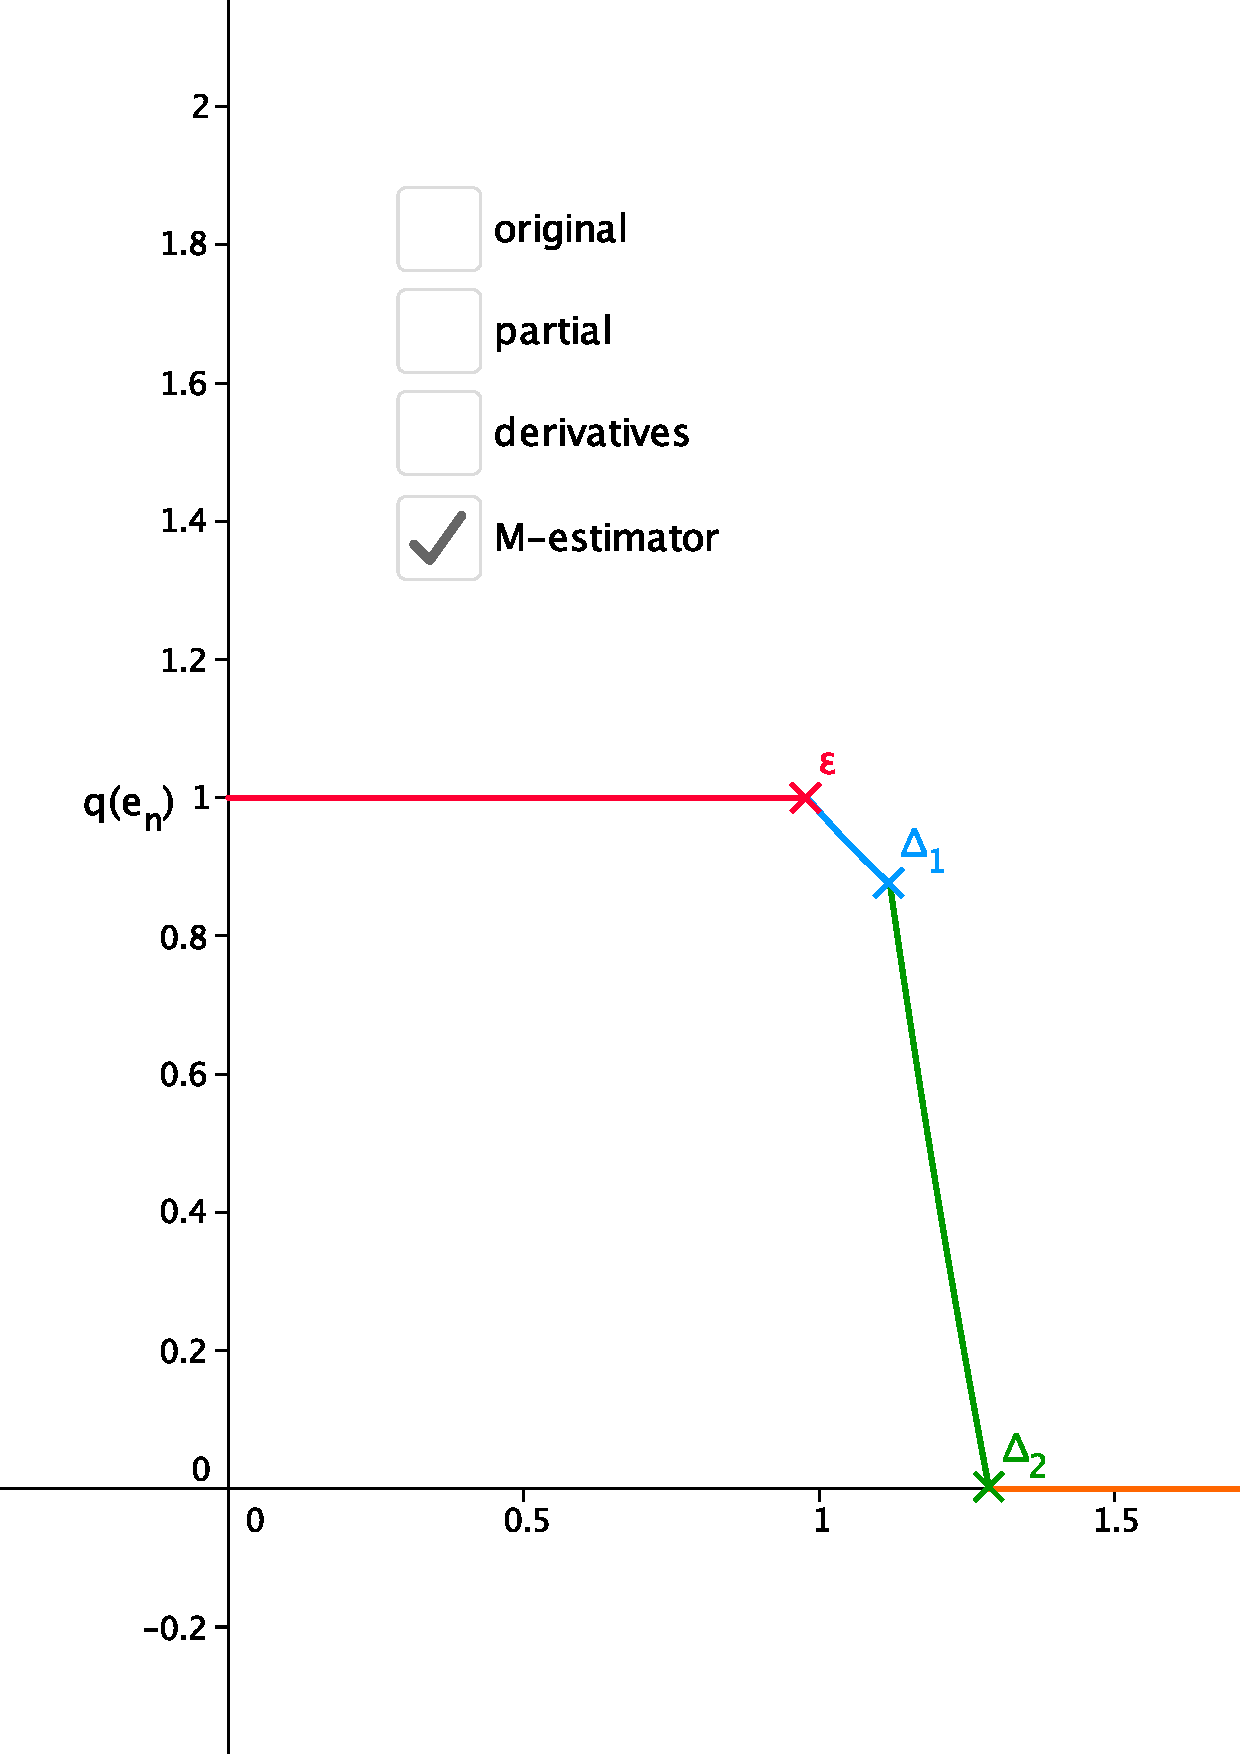
\includegraphics[width=\textwidth]{./images/m_estimate_q.pdf}
    \caption{Graph zu $q(e_n)$ bei einer Standardabweichung von $\sigma_n = 0.5$.}
    \label{fig:m-estimate-q}
\end{figure}
Wenn $q(e_n) = 1$ gilt, verhält sich der RLM genau wie der RLS, da die Gleichungen (\ref{eq:rlm:rls:bd}) und (\ref{eq:rlm:rlm:bd}) dann gleich sind. Für alle Werte $0 < q(e_n) < 1$ ergeben sich beim RLM kleinere Werte für $b$ und $d$ als beim RLS. Sollte $q(e_n) = 0$ gelten, so wird der aktuelle Fehler nicht in das Update von $\alpha_n$ und $S_n$ miteinbezogen, da dann $b=d=0$ gilt (vergleiche dazu Formeln (\ref{eq:rlm:rls:alpha}) und (\ref{eq:rlm:rls:s})). 
Kleine $q$-Werte sorgen also für eine Hemmung des aktuellen Fehlers auf die Updates von $\alpha_n$ und $S_n$.
In anderen Worten fomuliert: große Fehler beeinflussen das Update von $\alpha_n$ und $S_n$ weniger, als kleine Fehler.

Als Vorrausetzung gilt folglich, dass Impulse bzw. Ausreißer das Lernverhalten nicht beeinflussen sollen. Diese Annahme muss vom jeweiligen Anwendungsszenario abhängig gemacht werden, da es ggf. wünschenswert ist auf Ausreißer Rücksicht zu nehmen. In solchen Szenarien ist von der Verwendung des RLM abzuraten (für eine detallierte Diskussion siehe Abschnitt (\ref{sec:perf:bewertung})).

Maßgeblich für die Entscheidung ob der aktuelle Fehler als Impuls aufgefasst werden kann oder nicht sind die Grenzen $\xi$, $\Delta_1$ und $\Delta_2$ von $\rho(e_n)$. Wie in Abb. (\ref{fig:m-estimate-q}) zu sehen, bedeutet ein Fehler kleiner als $\xi$, dass sich der Algorithmus wie der RLS verhält, wohingegen ein Fehler größer als $\Delta_2$ dafür sorgt, dass beim Update von $\alpha_n$ und $S_n$ keine Rücksicht auf den Fehler genommen wird.
Die Grenzen müssen so gesetzt werden, dass mit ihnen Impulse von normalen Datensätzen unterschieden werden können.
Beim RLM-Algorithmus werden die Grenzen in jeder Iteration neu festgelegt. Als Basis dient die Standardabweichung der letzten $N$ Datensätze. Es werden nachfolgende Eigenschaften festgelegt, die besagen wieviel Prozent der Daten von den jeweiligen Grenzen miteinbegriffen werden sollen:
\begin{align}
    95\%& \quad \text{der Daten} \leq \xi \nonumber\\
    5\%& \quad \text{der Daten} > \xi \nonumber\\
    2.5\%& \quad \text{der Daten} > \Delta_1 \nonumber\\
    1\%& \quad \text{der Daten} > \Delta_2 \nonumber
\end{align}
Daraus können die folgenden direkten Abhängigkeiten der Grenzen zur Standardabweichung $\sigma_n$ getroffen werden:
\begin{align}
    \label{eq:rlm:rlm:limits}
    \xi =& 1.96 \cdot \sigma_n \nonumber\\
    \Delta_1 =& 2.24 \cdot \sigma_n \\
    \Delta_2 =& 2.576 \cdot \sigma_n \nonumber
\end{align}
Die Varianz wird mit folgender Formel errechnet:
\begin{align*}
    \hat{\sigma}^2_n = \lambda_\sigma\hat{\sigma}^2_{n-1} + C_1(1-\lambda_\sigma)\cdot \text{median}(A_n)) \quad\quad \text{mit}  \quad C_1 = 1.483(1+\frac{5}{N-1})
\end{align*}
$A_n = \{e^2_n, \ldots, e^2_{n-N+1}\}$ ist eine Menge der vergangenen $N$ quadrierten Fehler, $\lambda_\sigma$ ist ein zusätzlicher Vergessenheitsfaktor und $C_1$ eine Konstante um die Werte für die Berechnung von $\hat{\sigma}^2_n$ anzupassen.
Die aktuelle Varianz $\hat{\sigma}^2_n$ errechnet sich grob betrachtet aus der vorherigen Varianz $\hat{\sigma}^2_{n-1}$ und dem Median der letzten $N$ Fehler. Durch die Verwendung des Medians gehen \emph{vereinzelte} Ausreißer folglich nicht in die Berechnung der aktuellen Varianz mit ein. 
Dadurch soll erzielt werden, dass die Varianz lediglich das Rauschen erfasst und somit $\xi$, $\Delta_1$ und $\Delta_2$ Impulsfrei festgelegt werden können. Es ist anzumerken, dass auf Grenzen/Probleme der beschriebenen Berechnungen in Abschnitt (\ref{sec:performance}) näher eingegangen wird.

\subsubsection{Ablauf und Implementation}
\label{sec:rlm:rlm:implementation}
Dieser Abschnitt behandelt den eigentlichen Ablauf des RLM. Verknüpfend wird hier Bezug auf dessen Implementation in Matlab genommen.
Der Algorithmus ist als Bestandteil der \emph{UOSLib} \cite{UOSLib2013} geschrieben. In der Datei \texttt{icl\_initILS\_RLM.m} (siehe Anh. (\ref{apx:matlab:init})) werden Initialisierungen des RLM vorgenommen und in \texttt{icl\_learn\_RLM.m} (siehe Anh. (\ref{apx:matlab:learn})) befindet sich der Code, welcher in jeder Iteration des Lernprozesses ausgeführt wird.

In Tab. (\ref{tbl:rlm:rlm:impl:params}) sind alle vorgestellten Parameter des RLM aufgeführt samt deren Entsprechungen im Code und ihrer default-Werte. 
\begin{table}[H]
    \center
    \begin{tabular}{ | l | l | l | l |}
    \hline
    \textbf{Name} & \textbf{Symbol} & \textbf{Code} & \textbf{Defaultwert} \\ \hline \hline
    Vergessenheitsfaktor & $\lambda$ & \texttt{ILS.g} & 1\\ \hline
    Korrelationsmatrix & $S_0$ & \texttt{ILS.S} & \texttt{$10^5$*eye(length($x_0$))} \\ \hline
    \# Fehler im Median& $N$ & \texttt{ILS.errhist} & $30$\\ \hline
    Standardabweichung & $\sigma_0$ & \texttt{ILS.dev} & $1$ \\ \hline
    Vergessenheitsfaktor Median & $\lambda_\sigma$ & \texttt{ILS.gdev} & $0.9$ \\ \hline
    \end{tabular}
    \caption{Parameter des RLM samt deren Entsprechungen im Matlab-Code und ihrer default-Werte.}
    \label{tbl:rlm:rlm:impl:params}
\end{table}
In der Initialisierungsphase werden zunächst alle Parameter gesetzt. Die Wahl der Parameter kann explizit durch den Anwender geschehen, oder wird, sofern dieser keine Werte festlegt, mit default-Werten getan. Anschließend werden die Grenzen $\xi$ ($\widehat{=}$\texttt{ILS.eps}), $\Delta_1$ ($\widehat{=}$\texttt{ILS.delta\_1}) und $\Delta_2$ ($\widehat{=}$\texttt{ILS.delta\_2}) entsprechend der Standardabweichung initialisiert.
\\\\
Der Ablauf des Lernprozesses in einer Iteration lässt sich wie folgt zusammenfassen:
\begin{enumerate}\itemsep0pt \parskip0pt \parsep0pt
  \item Aufruf von \texttt{icl\_learn\_RLM} mit aktueller Parameterkonfiguration in \texttt{ILS}, dem Datenpunkt \texttt{x}, dem vorhergesagten Wert \texttt{yp} und echten Wert \texttt{y}
  \item Der aktuelle Fehler \texttt{e\_n} wird berechnet
  \item \texttt{x\_n} wird auf Basisfunktionen angewendet
  \item $q(e_n)$ wird mittels der Funktion \texttt{m\_estimate(e\_n, ILS)} basierend auf Fehler \texttt{e\_n} und aktuellen Grenzen in \texttt{ILS} angewendet und Wert in \texttt{q\_n} abgelegt
  \item Der \texttt{gain}-Vektor wird berechnet
  \item Der $\alpha_n$ Vektor wird aktualisiert
  \item Die Adaptionsmatrix $S_n$ wird aktualisiert
  \item Die neue Standardabweichung $\sigma_{n+1}$ wird berechnet und \texttt{ILS.eps}, \texttt{ILS.delta\_1} und \texttt{ILS.delta\_2} werden neu gesetzt.
\end{enumerate}
Bei den Updates von $\alpha_n$ und $S_n$ weicht der Code von der in der Ausarbeitung verwendeten Formeln ein wenig ab, verändern das Resultat jedoch nicht. Anstelle der in den Gleichungen (\ref{eq:rlm:rls:alpha}) und (\ref{eq:rlm:rlm:s}) verwendeten Variablen $b$ und $d$ wird in der Implementation der gain-Vektor berechnet und in den Update-Formeln verwendet (vergleiche dazu mit den Zeilen 41 und 44 in in Anh. (\ref{apx:matlab:learn})). Der Code orientiert sich stärker an der Herangehensweies von \cite{zou2000recursive}, während diese Ausarbeitung mit Hinsicht auf Konsistenz mit den Vorbereitungsfolien geschrieben wurde.

Zur Performance-Evaluierung von impulsversetzten Daten (siehe Abschnitt (\ref{sec:perf:impulse})) existiert eine weitere Funktion, welche in \texttt{icl\_base} aufgerufen wird um Offsets auf bestimmte Datensätze zu addieren. Die Methode \texttt{icl\_genImpulses} (siehe Anh. (\ref{apx:matlab:imp})) nimmt als Parameter das Datenset und addiert Offsets, welche als weitere Parameter der Funktion übergeben werden können. Es sind nicht alle Funktionalitäten fertiggestellt, da die option \texttt{impulseArray} für die Evaluierung ausgereicht hat.

\section{Performance}
\label{sec:performance}
In diesem Abschnitt wird auf die Performance des RLM in verschiedenen Szenarien eingegangen. Jedes Szenario wird zum Vergleich sowohl mit dem RLM als auch mit dem RLS durchlaufen. Dies soll helfen den RLM besser vom RLS abgrenzen zu können und ihn somit leichter in einen Kontext einordnen zu können. 

Die verwendeten Maße zur Messung der Performance sind
\begin{align}
  e_c(T) &= \sum_{t=1}^{T} L(f(x_t,\alpha_t),y_t) & \text{Kumulativer Loss}\nonumber\\
  e_d(T) &= \sum_{t=1}^{T} L(f(x_t,\alpha_T),y_t) & \text{Loss auf allen Daten}\nonumber\\
  e_g(T) &= \sum_{x \in X} L(f(x,\alpha_T),y_t) & \text{Loss auf Zielfunktion}\nonumber
\end{align}
Sofern nicht anders in dem jeweiligen Anwendungsfall angegeben, ist das Standardsetup des RLM und des RLS wie in Tab. (\ref{tbl:perf:setup}) angegeben.
\begin{table}[H]
    \center
    \begin{tabular}{| l | l | l |}
    \hline
    \textbf{Parameter} & \textbf{RLM} & \textbf{RLS} \\ \hline \hline
    $S$ & 10000 & 10000 \\ \hline
    $\lambda$ & 0.99 & 0.99 \\ \hline
    $\lambda_\sigma$ & 0.85 & - \\ \hline
    $N$ & 15 & - \\ \hline
    $\sigma_0$ & 1 & - \\ \hline
    \end{tabular}
    \caption{Default-Setup des RLM/RLS.}
    \label{tbl:perf:setup}
\end{table}

Zu Beginn wird in Abschnitt (\ref{sec:perf:ausdruck}) auf Szenarien mit Approximatoren verschiedener Ausdrucksstärken eingegangen. Dort soll auch eine Einführung in das allgemeine Approximationsverhalten des RLM gegeben werden. Anschließend werden in Teil (\ref{sec:perf:rauschen}) Ergebnisse vorgestellt, welche den Umgang des RLM mit verrauschten Daten beschreiben. In Abschnitt (\ref{sec:perf:trajektorien}) wird die Wirkung von Trajektorieneffekten in den Daten erörtert. Danach werden zeitvariante Zielfunktionen betrachtet (Abschnitt (\ref{sec:perf:zeitvarianz})). Im Anschluss wird auf nichtlineare Zielfunktionen eingegangen (Abschnitt (\ref{sec:perf:nichtlinear})). Beim letzten Szenario in Abschnitt (\ref{sec:perf:impulse}) wird auf die Ergebnisse des RLM bei impulsversetzten Daten eingegangen. Zum Schluss werden die erarbeiteten Ergebnisse in Beziehung gebracht und bewertet und mit einem anderen robusten Lernverfahren, dem PRRLS, verglichen.

\subsection{Ausdrucksstärke}
\label{sec:perf:ausdruck}
Als Setup\footnote{\textbf{Setup}:\quad\texttt{Zielfunktion=poly, \# Datensätze=100, \# Groundtruth=100, noise=0.0, minpath=false, Approximator=Polynom Grad 6}} wird eine polynomielle Zielfunktion mit einem Polynom 6. Grades approximiert.
In den Abb. (\ref{fig:perf:ausdruck:ausdruck3}), (\ref{fig:perf:ausdruck:ausdruck4}), (\ref{fig:perf:ausdruck:ausdruck9}) und (\ref{fig:perf:ausdruck:ausdruck16}) sind die Approximationen von RLM und RLS nach 3, 4, 9 und 16 Lerndaten zu sehen.
\begin{figure}[H]
  \centering
  \begin{subfigure}[b]{0.4\textwidth}
    \centering
    \includegraphics[width=\textwidth]{./images/copyofstats/ausdruck6_approx_piece_3.eps}
    \caption{Approximation nach 3 Daten.}
    \label{fig:perf:ausdruck:ausdruck3}
  \end{subfigure}
  \begin{subfigure}[b]{0.4\textwidth}
    \centering
    \includegraphics[width=\textwidth]{./images/copyofstats/ausdruck6_approx_piece_4.eps}
    \caption{Approximation nach 4 Daten.}
    \label{fig:perf:ausdruck:ausdruck4}
  \end{subfigure}
  \\
  \begin{subfigure}[b]{0.4\textwidth}
    \centering
    \includegraphics[width=\textwidth]{./images/copyofstats/ausdruck6_approx_piece_9.eps}
    \caption{Approximation nach 9 Daten.}
    \label{fig:perf:ausdruck:ausdruck9}
  \end{subfigure}
  \begin{subfigure}[b]{0.4\textwidth}
    \centering
    \includegraphics[width=\textwidth]{./images/copyofstats/ausdruck6_approx_piece_16.eps}
    \caption{Approximation nach 16 Daten.}
    \label{fig:perf:ausdruck:ausdruck16}
  \end{subfigure}
  \\
  \caption{}
  \label{fig:perf:ausdruck:approx}
\end{figure}
Bis zum dritten Lerndatum verhalten sich beide Lernverfahren gleich, was in Abb. (\ref{fig:perf:ausdruck:ausdruck3}) an den übereinanderliegenden Graphen erkennbar ist. Beim vierten Lerndatum (siehe Abb. (\ref{fig:perf:ausdruck:ausdruck4})) ist zu sehen, dass sich beide Lernverfahren nun unterschiedlich verhalten. Während der RLS das präsentierte Lerndatum abbildet, zeigt der RLM keine Veränderung gegenüber Schritt 3. Der Grund für dieses Verhalten lässt sich anschaulich an Abb. (\ref{fig:perf:ausdruck:ausdruck4}) zeigen. Der Fehler $e_n$ zwischen der approximierten Kurve des RLM und des neuen Lerndatums ist "`hoch"'. Bei einem "`hohen"' Fehler wird $q(e_n)$ auf 0 gesetzt und hemmt somit das Update von $\alpha_n$ und $S_n$. Als Resultat zeigt der Graph des RLM in Schritt 4 also dieselbe Approximation wie im Schritt zuvor.

Dieses Verhalten ist stark von den gewählten Parametern abhängig und kann dementsprechend beeinflusst werden. Da die Grenzen $\xi$, $\Delta_1$ und $\Delta_2$ steuern, ab wann ein Fehler als "`hoch"' zu betrachten ist und diese wiederum abhängig von der Standardabweichung sind, kann  $\sigma_0$ größer gewählt werden, sodass $q$ den auftretenden Fehler in Schritt 4 nicht mit 0 bewertet und somit ein Update von $\alpha_n$ und $S_n$ zulässt.

Eine weitere Möglichkeit ist, dass Updateverhalten der Standardabweichung zu verändern. Mittels dem Vergessenheitsfaktor $\lambda_\sigma$ kann bestimmt werden, wie sehr die Standardabweichung neue Fehler mit einschließt. Wird der Wert "`klein"' gewählt, so hat der Median der vergangenen Fehlerwerte "`größeren"' Einfluss auf $\sigma$ (siehe Gleichung (\ref{eq:rlm:rlm:limits})). Hier ist zu beachten, dass diese Veränderung das Update von $\sigma$ lediglich weniger träge macht. Es bedeutet nicht, dass jeder Fehler sofort die Standardabweichung beeinflusst, da diese weiterhin abhängig vom Median der vergangenen Fehlerwerte ist.

Es gibt eine weitere Möglichkeit das Approximationsverhalten in dem Szenario in Abb. (\ref{fig:perf:ausdruck:approx}) zu variieren. Eine Änderung in der Anzahl der vergangenen Fehler $N$ über welche der Median gebildet wird, kann dafür sorgen, dass der Median schneller bzw. langsamer auf Fehler reagiert. Denn damit z.B. große Fehler vom Algorithmus beachtet werden sollen, müssen diese mindestens $\left\lceil \frac{N}{2} \right\rceil$ der Objekte ausmachen über die der Median gebildet wird. Wenn also $N$ "`klein"' gewählt wird, haben wenige Fehler bereits die Möglichkeit Einfluss auf $\sigma$ zu nehmen.

Ab Lernschritt 9 lässt sich Abb. (\ref{fig:perf:ausdruck:ausdruck9}) erkennen, dass der RLS, im Gegensatz zum RLM, die unterliegende Funktion bereits gut angenähert hat. Der RLM verbleibt weitere 4 Lerndaten in dieser Form, bis zu dem Punkt, wo ein Datum nah genug an seiner Approximation liegt, sodass der Fehler klein genug ist um ein Update zu ermöglichen. 
Dieses Verhalten wird ebenfalls in den Szenarien der Abschnitte (\ref{sec:perf:trajektorien}) und (\ref{sec:perf:nichtlinear}) besprochen. Schlussendlich liegt der RLM nach dem 16. Lerndatum wieder Deckungsgleich auf dem RLS.

Nun sollen die Performance-Ergebnisse der besprochenen Approximationen betrachtet werden. In Abb. (\ref{fig:perf:ausdruck:perf16}) sind die Werte der einzelnen Performancemaße der 16 Lerndaten zu sehen.
\begin{figure}[H]
        \centering
        \begin{subfigure}[b]{0.4\textwidth}
                \centering
                \includegraphics[width=\textwidth]{./images/copyofstats/ausdruck6_perf_piece_9.eps}
                \caption{Performance nach 9 Daten.}
                \label{fig:perf:ausdruck:perf9}
        \end{subfigure}
        \begin{subfigure}[b]{0.4\textwidth}
                \centering
                \includegraphics[width=\textwidth]{./images/copyofstats/ausdruck6_perf_piece_16.eps}
                \caption{Performance nach 16 Daten.}
                \label{fig:perf:ausdruck:perf16}
        \end{subfigure}
        \\
        \caption{}
        \label{fig:perf:ausdruck:perf}
\end{figure}
Beim dritten Lerndatum liegen die Kurven beider Lernverfahren in jedem Performancemaß übereinander, wie auch in der Approximation erkennbar ist. Da der Approximator mit Grad 6 in der Lage ist die bereits präsentierten Daten abzubilden zeigt der Loss auf den vergangenen Daten keinen Anstieg. Der Fehler zu den GroundTruth-Daten steigt hier jedoch an. Der Grund für dieses Verhalten ist, dass bisher ausschließlich die 3 Datensätze abbgebildet werden sollten und wie in Abb. (\ref{fig:perf:ausdruck:ausdruck3}) zu erkennen ist, jedoch diese Informationen nicht ausreichen um die GroundTruth-Funktion anzunähern.
In Schritt 4 verhalten sich beide Algorithmen unterschiedlich, was auch in den Performance-Werten sichtbar wird (siehe Abb. (\ref{fig:perf:ausdruck:perf9})). Da der RLM den neuen Datenpunkt nicht abbildet, steigt der Loss auf den vergangenen Datensätzen. Durch die unveränderte Konfiguration seiner Parameter bleibt der Loss auf den GroundTruth-Daten gleich. Dieser Effekt lässt sich ebenfalls ab dem neunten Lerndatum wiederfinden. Wie in Abb. (\ref{fig:perf:ausdruck:perf16}) zu sehen ist steigt der Previous-Data Loss bis zum 13 Lerndatum an. Solange werden Daten präsentiert, bei welchen der Fehler so groß ist, dass der RLM diese als Impulse einschätzt und somit keine Adaption herbeiführt. Erst das 14. Lerndatum liegt nah genug an der Approximation, sodass der RLM eine Adaption vornimmt und somit die vergangenen Daten besser abbildet.\\
Für die restlichen 94 Lerndaten verhalten sich RLM und RLS gleich, da beide die GroundTruth-Funktion ab Lerndatum 16 abbilden.

Es wurde ein weiteres Setup\footnote{\textbf{Setup}:\quad\texttt{Zielfunktion=poly, \# Datensätze=100, \# Groundtruth=100, noise=0.0, minpath=false, Approximator=Polynom Grad 1}} getestet, welches einen linearen Approximator auf polynomiellen GroundTruth-Daten anwendet (siehe Anh. (\ref{fig:apx:ausdruck:ausdruck11}) und (\ref{fig:apx:ausdruck:perf11})). Es ist zu beobachten, dass sich die Performance-Ergebnisse beider Verfahren nicht sehr unterscheiden. Der Grund hierfür ist, dass mittels eines linearen Approximators der Fehler zu den präsentierten Daten kleiner bleibt, als bei einem Polynom höheren Grades. Dadurch wird die Hemmung klein gehalten, wodurch das Verhalten des RLM stark dem des RLS ähnelt.

Zusammenfassend lässt sich sagen, das ein Approximator mit einer hohen Ausdrucksstärke dazu führt, dass die initiale Phase in der der RLS sich auf die Zielfunktion einpendeln muss, verlängert wird, da Lerndaten fälschlicherweise als Ausreißer interpretiert werden. Die Performance nach der initialen Phase verhält sich gleich wie beim RLS.

\subsection{Rauschen}
\label{sec:perf:rauschen}
In diesem Abschnitt werden RLM und RLS in zwei Setups auf verrauschten Daten angewendet.

Beim ersten Setup\footnote{\textbf{Setup}:\quad\texttt{Zielfunktion=linear, \# Datensätze=100, \# Groundtruth=100, noise=0.1, minpath=false, Approximator=Polynom Grad 1}} wird ein linearer Approximator und eine lineare Zielfunktion verwendet, welche dem Lernverfahren verrauscht präsentiert wird. Wie in den Abb. (\ref{fig:perf:rauschen1}) erkennbar ist, sind Approximierung und Performance des RLM und RLS identisch.
\begin{figure}[H]
        \centering
        \begin{subfigure}[b]{0.4\textwidth}
                \centering
                \includegraphics[width=\textwidth]{./images/copyofstats/rauschen1_approx_100.eps}
                \caption{}
                \label{fig:perf:rauschen1:approx}
        \end{subfigure}
        \begin{subfigure}[b]{0.4\textwidth}
                \centering
                \includegraphics[width=\textwidth]{./images/copyofstats/rauschen1_perf_100.eps}
                \caption{}
                \label{fig:perf:rauschen1:perf}
        \end{subfigure}
        \\
        \caption{Approximation und Performance-Ergebnisse bei linearem Approximator auf linearen GroundTruth-Daten mit Rauschen.}
        \label{fig:perf:rauschen1}
\end{figure}
Verrauschte Daten resultieren beim RLM in einer größeren Standardabweichung, sodass die auftretenden Fehlerwerte, trotz Rauschen, nicht zu einer Hemmung des Parameterupdates führen.

Das zweite Setup\footnote{\textbf{Setup}:\quad\texttt{Zielfunktion=linear, \# Datensätze=100, \# Groundtruth=100, noise=0.1, minpath=false, Approximator=Polynom Grad 5}} soll diesen Aspekt anhand eines polynomiellen Approximators 5. Grades untersützen und zusätzlich einige Inhalte aus Abschnitt (\ref{sec:perf:ausdruck}) erneut verdeutlichen.
\begin{figure}[H]
        \centering
        \begin{subfigure}[b]{0.4\textwidth}
                \centering
                \includegraphics[width=\textwidth]{./images/copyofstats/rauschen5_approx_100.eps}
                \caption{}
                \label{fig:perf:rauschen5:approx}
        \end{subfigure}
        \begin{subfigure}[b]{0.4\textwidth}
                \centering
                \includegraphics[width=\textwidth]{./images/copyofstats/rauschen5_perf_100.eps}
                \caption{}
                \label{fig:perf:rauschen5:perf}
        \end{subfigure}
        \\
        \caption{Approximation und Performance-Ergebnisse bei polynomiellen Approximator 5. Grades auf linearen GroundTruth-Daten mit Rauschen.}
        \label{fig:perf:rauschen5}
\end{figure}
Wie in Abb. (\ref{fig:perf:rauschen5:approx}) zu sehen ist, haben beide Lernverfahren nach 100 Datensätzen trotz hoher Ausdrucksstärke die Kurve relativ gut angenähert. Mit Hinblick auf die Performance-Ergebnisse in Abb. (\ref{fig:perf:rauschen5:perf}) lässt sich jedoch ein großer Unterschied feststellen. Der RLM zeigt einen hohen Loss bei allen Performancemaßen im Bereich vor dem 16. Lerndatum.
Grund für dieses Verhalten sind weniger die verrauschten Daten, als die hohe Ausdrucksstärke des Approximators. Für die Erklärung dieses Sachverhaltes sei auf das erste Setup in Abschnitt (\ref{sec:perf:ausdruck}) verwiesen.

Zusammenfassend lässt sich sagen, dass der RLM mit Rauschen keine Problem hat, solange die verrauschten Daten mit einer gewissen Varianz um die Zielfunktion liegen (z.B. Gauss-verteilt).

\subsection{Trajektorieneffekte}
\label{sec:perf:trajektorien}
In diesem Teil der Ausarbeitung wird auf Trajektorieneffekte bei den Lerndaten eingegangen. Es wird ein Setup\footnote{\textbf{Setup}:\quad\texttt{Zielfunktion=linear, \# Datensätze=100, \# Groundtruth=100, noise=0.0, minpath=true, Approximator=Polynom Grad 5}} vorgestellt in dem eine lineare Zielfunktion mit einem Polynom 5. Grades approximiert wurde. In Abb. (\ref{fig:perf:trajektorien5:approx}) ist zu sehen, dass sich RLM und RLS zu allen Zeitpunkten gleich verhalten.
\begin{figure}[H]
        \centering
        \begin{subfigure}[b]{0.4\textwidth}
                \centering
                \includegraphics[width=\textwidth]{./images/copyofstats/trajektorien5_approx_100.eps}
                \caption{}
                \label{fig:perf:trajektorien5:approx}
        \end{subfigure}
        \begin{subfigure}[b]{0.4\textwidth}
                \centering
                \includegraphics[width=\textwidth]{./images/copyofstats/trajektorien5_perf_100.eps}
                \caption{}
                \label{fig:perf:trajektorien5:perf}
        \end{subfigure}
        \\
        \caption{Approximation und Performance-Ergebnisse bei polynomiellen Approximator 5. Grades auf linearen GroundTruth-Daten mit Trajektorieneffekten.}
        \label{fig:perf:trajektorien5}
\end{figure}
Die Erklärung für dieses Verhalten liegt der Tatsache zugrunde, dass immer jenes Datum als nächstes präsentiert wird, welches die Eigenschaft hat, die kürzeste Distanz zum vorhergehenden Datum zu haben. Da der RLM, genau wie der RLS, versucht den Fehler zu allen Daten zu minimieren und in diesem Szenario, die Daten immer nahe an den vergangenen Daten liegen, führt dies dazu, dass die Fehlerwerte nur mit einer geringen Wahrscheinlichkeit groß werden. Diese Besonderheit sorgt dafür, dass das Verhalten nicht die gleichen hohen Loss-Werte wie bei dem Szenario aus Abschnitt (\ref{sec:perf:rauschen}) aufweist. Da keine Hemmung des Parameter- und Adaptionsupdates stattfindet, verhalten sich beide Algorithmen gleich.

Bei der Erklärung dieses Sachverhalts gilt die implizite Annahme, dass die Datendichte ausreichend hoch ist bzw. die Daten nicht sehr weit voneinander entfernt liegen. In beiden Fällen kann es passieren, dass die Abstände zum nächsten Lerndatum für einen zu hohen Fehler $e_n$ sorgen, welcher das Update von $\alpha_n$ und $S_n$ hemmt.

Mit Blick auf die Performancemaße in Abb. (\ref{fig:perf:trajektorien5:perf}) lässt sich sehen, dass beide Algorithmen mehr Zeit benötigen die Zielfunktion abzubilden als vergleichbare Szenarien der anderen Abschnitte. Dies liegt an der Tatsache, dass der Approximator anfänglich nur einen Teil der Zielfunktion annähern kann, während die Zielfunktion insgesamt auf einem größeren Intervall definiert ist, dem Algorithmus jedoch schlichtweg nicht bekannt ist zu Beginn.

Auf die Vorstellungen zweier weiterer Setups\footnote{\textbf{Setup}:\quad\texttt{Zielfunktion=linear, \# Datensätze=100, \# Groundtruth=100, noise=0.0, minpath=true, Approximator=Polynom Grad 1}}$^,$\footnote{\textbf{Setup}:\quad\texttt{Zielfunktion=linear, \# Datensätze=100, \# Groundtruth=100, noise=0.0, minpath=true, Approximator=Polynom Grad 3}} mit kleinerem Approximatorgrad wird hier verzichtet, da die sich Ergebnisse analog zu dem erstbeschriebenen Setup verhalten. Die Ergebnisse sind im Anhang in den Abb. (\ref{fig:apx:trajektorien1}) und (\ref{fig:apx:trajektorien3}) zu sehen.


\subsection{Zeitvarianz}
\label{sec:perf:zeitvarianz}
In diesem Abschnitt soll das Verhalten bei zeitvarianten Zielfunktionen erörtert werden.
Dazu wird wird ein Setup\footnote{\textbf{Setup}:\quad\texttt{Zielfunktion=relearn, \# Datensätze=100, \# Groundtruth=100, noise=0.0, minpath=false, Approximator=Polynom Grad 5}} mit zwei verschiedenen Vergessenheitsfaktoren $\lambda$ durchgeführt um dessen Einfluss auf die Approximation zu zeigen. Der Parameter wird in jeder Variante sowohl für den RLM als auch RLS gesetzt. Es ergeben sich die Approximationen in den Abb. (\ref{fig:perf:zeitvarianz:approx99}) und (\ref{fig:perf:zeitvarianz:approx95}) mit jeweils $\lambda=0.99$ (Standard-Setup) und $\lambda=0.95$.
\begin{figure}[H]
        \centering
        \begin{subfigure}[b]{0.4\textwidth}
                \centering
                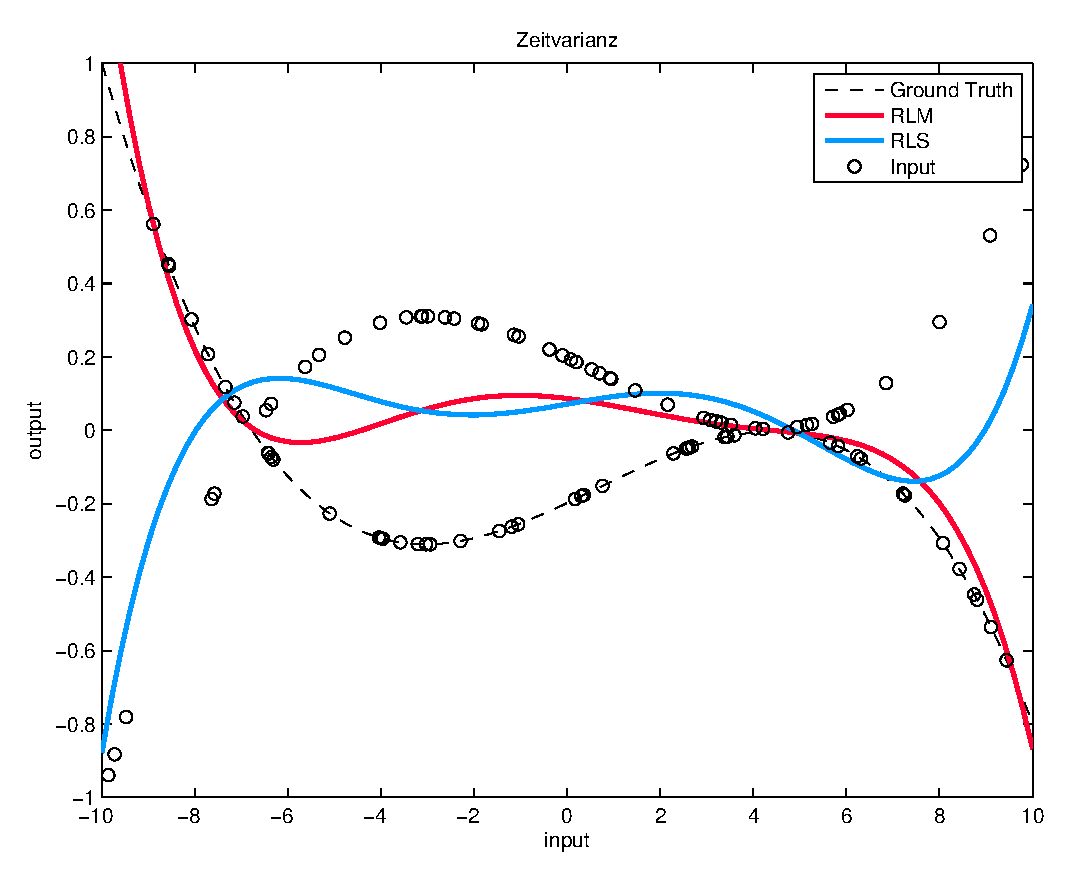
\includegraphics[width=\textwidth]{./images/copyofstats/zeitvarianz(99)5_approx_100.eps}
                \caption{$\lambda=0.99$}
                \label{fig:perf:zeitvarianz:approx99}
        \end{subfigure}
        \begin{subfigure}[b]{0.4\textwidth}
                \centering
                \includegraphics[width=\textwidth]{./images/copyofstats/zeitvarianz(95)5_approx_100.eps}
                \caption{$\lambda=0.95$}
                \label{fig:perf:zeitvarianz:approx95}
        \end{subfigure}
        \\
        \caption{Approximation und Performance-Ergebnisse bei polynomiellen Approximator 5. Grades auf zeitvarianter Zielfunktion mit unterschiedlichem $\lambda$.}
        \label{fig:perf:zeitvarianz}
\end{figure}
In diesem Szenario kommt die erste Hälfte der Lerndaten $(=50)$ von der gestrichelten Zielfunktion und die zweite Hälfte von ihrer Spiegelung an der x-Achse (schemenhaft an den Punkten in beiden Graphen erkennbar).

Es lässt sich sagen, dass dieses Szenario eine Herausforderung für RLS und RLM darstellt, da diese den Fehler auf allen Lerndaten zu minimieren. Folglich versuchen beim Umschalten der Zielfunktion beide Lernverfahren die alte Zielfunktion abzubilden, werden jedoch durch erhöhte Fehlerraten dazu geführt sich der neuen Zielfunktion anzupassen. Dieses Verhalten kann durch variieren des Vergessenheitsfaktors beschleunigt werden. Dazu wird zunächst Abb. (\ref{fig:perf:zeitvarianz:approx99}) betrachtet. Im Intervall $[-6,8]$ verhalten sich beide Graphen relativ ähnlich, wohingegen in den Randgebieten der RLS die neue Zielfunktion und der RLM die alte Zielfunktion abbildet.
Erneut liegt dies an der Fehlergröße, welche in den Randgebieten, aufgrund der großen Distanz zwischen den Lerndaten der alten und neuen Zielfunktion, zu einer Hemmung der Anpassung des RLM sorgt.
Auch ein kleinerer $\lambda$-Wert hat hier keinen Einfluss auf dieses Verhalten, da, wie in Abb. (\ref{fig:perf:zeitvarianz:approx95}) erkennbar, zwar im mittleren Teil eine klare Näherung der neuen Funktion stattfindet, in den Randgebieten jedoch keine essentielle Änderung zu sehen ist.
Genau diese Situation ist problematisch für den RLM. Denn der Teil, der gut vom RLM abgebildet wird ist viel größer als der Teil der schlecht vom RLM abgebildet wird. Folglich werden die Fehlerwerte für die meisten Lerndaten relativ gering sein, was zu einer geringen Standardabweichung führt. Dementsprechend entsteht in den Randgebieten das Problem, dass den dortigen Fehlern immer weniger Bedeutung im Parameter- und Adaptionsupdate zugesprochen wird, da die Wahrscheinlichkeit mit der diese Fehler $\left\lceil \frac{N}{2} \right\rceil$-Mal kurz hintereinander auftreten, aufgrund der geringen Größe der problematischen Bereiche, gering ist. Diesem Problem kann entegegengewirkt werden, indem $N$ kleiner gewählt wird (Erklärung zu diesem Sachverhalt analog in Abschnitt (\ref{sec:perf:ausdruck})).

\subsection{Nichtlinearität}
\label{sec:perf:nichtlinear}

In diesem Abschnitt geht auf das Verhalten des RLM bei nichtlinearen Zielfunktionen ein.
Im Setup\footnote{\textbf{Setup}:\quad\texttt{Zielfunktion=nonlin, \# Datensätze=100, \# Groundtruth=100, noise=0.0, minpath=false, Approximator=GLT lin}} wird ein lokaler Approximator mit 14 Stützstellen auf einer nichtlinearen Zielfunktion angewendet. Wie in Abb. (\ref{fig:perf:nichtlinear:perf}) zu sehen ist, sind die Loss-Werte zwar unterschiedlich, spielen sich jedoch in einem relativ niedrigen Zahlenbereich ab.
\begin{figure}[H]
        \centering
        \begin{subfigure}[b]{0.4\textwidth}
                \centering
                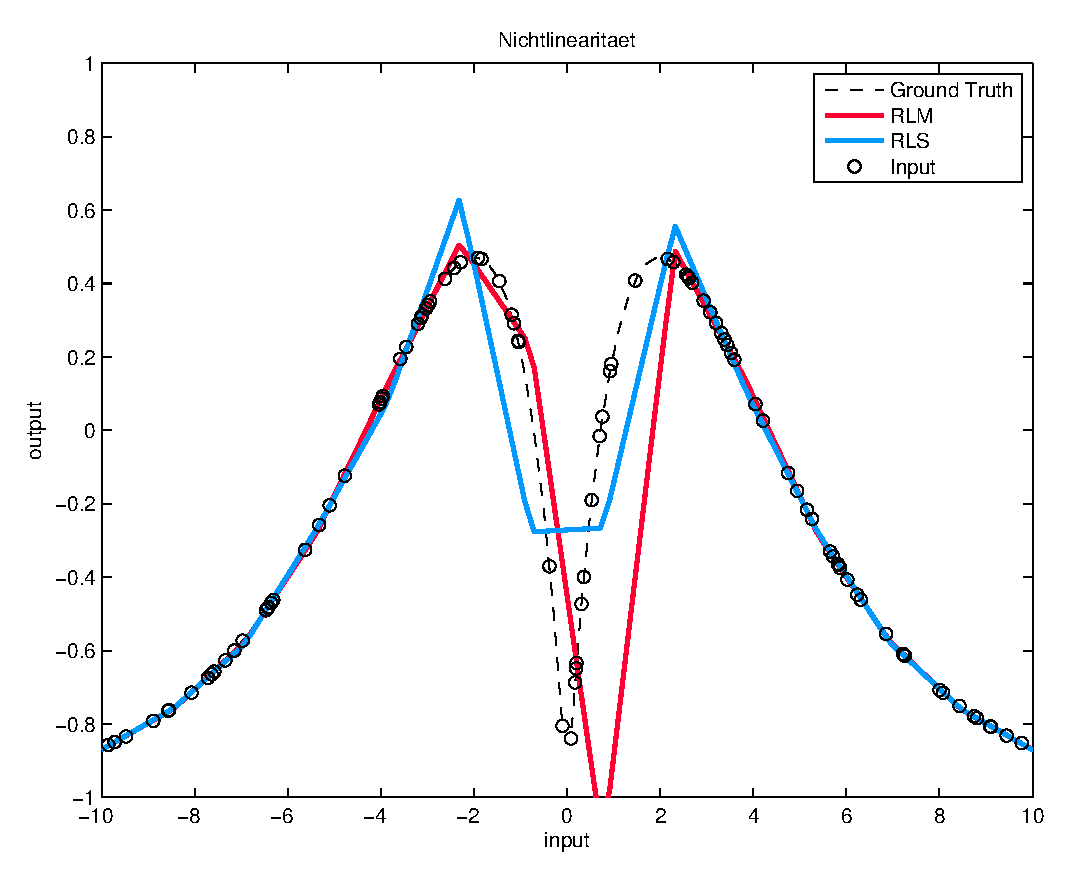
\includegraphics[width=\textwidth]{./images/copyofstats/nonlin14_approx_100GLT.eps}
                \caption{}
                \label{fig:perf:nichtlinear:approx}
        \end{subfigure}
        \begin{subfigure}[b]{0.4\textwidth}
                \centering
                \includegraphics[width=\textwidth]{./images/copyofstats/nonlin14_perf_100GLT.eps}
                \caption{}
                \label{fig:perf:nichtlinear:perf}
        \end{subfigure}
        \\
        \caption{Approximation und Performance-Ergebnisse bei lokalem linearem Approximator auf nichtlinearer Zielfunktion.}
        \label{fig:perf:nichtlinear}
\end{figure}
Das unterschiedliche Verhalten beider Verfahren hängt erneut mit der fehlerhaften Erkennung von Impulsen in den regulären Lerndaten zusammen.

Auf ein weiteres Setup\footnote{\textbf{Setup}:\quad\texttt{Zielfunktion=nonlin, \# Datensätze=100, \# Groundtruth=100, noise=0.0, minpath=false, Approximator=Polynom Grad 3}} mit einem globalen Approximator 3. Grades wird hier verzeichtet und lediglich auf die Ergebnisse im Anhang verwiesen, da daraus keine neuen Erkentnisse zu ziehen sind (siehe Abb. (\ref{fig:apx:nichtlinear}) im Anhang).

\subsection{Impulse}
\label{sec:perf:impulse}
Dieser Teil der Ausarbeitung behandelt das Verhalten des RLM auf impulsversetzten Daten.
Wenn vereinzelt Ausreißer in den Lerndaten vorkommen, so werden diese aufgrund des hohen auftretenden Fehlers $e_n$ ignoriert. Der Umgang des RLM mit hohen Fehlern wurde mehrfach in den vorigen Abschnitten diskutiert, daher werden hier zwei Sonderfälle betrachtet, welche Grenzen und Besonderheiten des RLM aufzeigen.
Zuerst werden Impulse betrachtet, welche in der initialen Phase des RLM auftreten und anschließend die Wirkung von aufeinanderfolgenden Ausreißern diskutiert.

\subsubsection{Impulse in Initialphase}
\label{sec:perf:impulse:intial}
Als Setup\footnote{\textbf{Setup}:\quad\texttt{Zielfunktion=poly, \# Datensätze=100, \# Groundtruth=100, noise=0.0, minpath=false, Approximator=Polynom Grad 4}} wird ein polynomieller Approximator 4. Grades auf eine polynomielle Zielfunktion angewendet. Die Lerndaten zu den Zeitpunkten $4$ und $10$ sind jeweils mit einem Offset von $-10$ versehen worden und befinden sich an den Stellen $(-3.2080|-10.3208)$ und $(-7.1535|-10.7153)$. 
In Abb. (\ref{fig:perf:impinit:approx}) ist sichtbar, dass der RLS die Zielfunktion schlechter annähert als der RLM.
\begin{figure}[H]
        \centering
        \begin{subfigure}[b]{0.4\textwidth}
                \centering
                \includegraphics[width=\textwidth]{./images/copyofstats/impsuperinit(dev5)_approx_100.eps}
                \caption{}
                \label{fig:perf:impinit:approx}
        \end{subfigure}
        \begin{subfigure}[b]{0.4\textwidth}
                \centering
                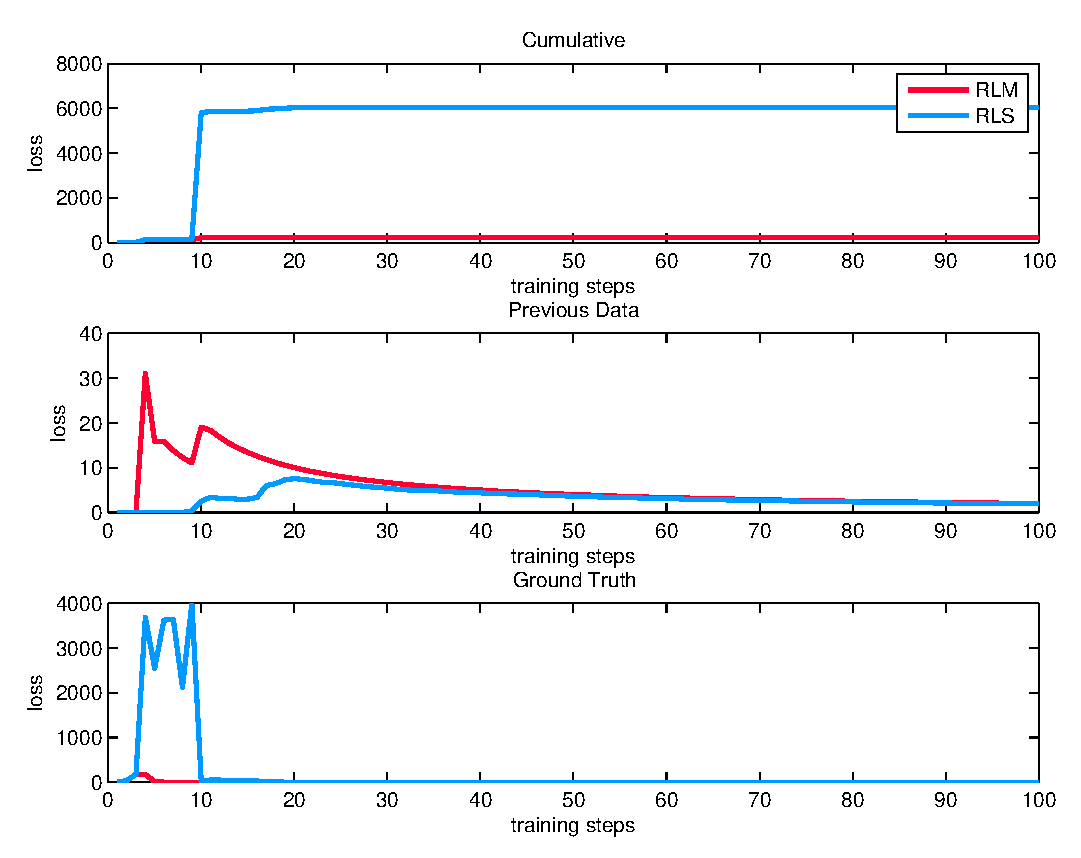
\includegraphics[width=\textwidth]{./images/copyofstats/impsuperinit(dev5)_perf_100.eps}
                \caption{}
                \label{fig:perf:impinit:perf}
        \end{subfigure}
        \\
        \caption{Approximation und Performance-Ergebnisse bei polynomiellem Approximator 4. Grades auf impulsversetzten Daten in der initialen Phase.}
        \label{fig:perf:impinit}
\end{figure}
Der RLS versucht den quadrierten Fehler zu allen Daten zu minimieren, also auch zu den Impulsen. Der RLM hingegen ignoriert diese beiden Ausreißer. In Abb. (\ref{fig:perf:impinit:perf}) lässt sich das Verhalten beider Algorithmen nachvollziehen.
Zu Zeitpunkt 4 und 10 wird der Loss des RLM auf den vergangenen Daten hoch, da er diese nicht abbildet. Der Loss auf die GroundTruth-Daten bleibt dementsprechend gering. Beim RLS verhalten sich die Performancemaße genau andersherum. Durch das Abbilden der Impulse bleibt der Previous-Data Loss gering, jedoch steigt der Loss auf den GroundTruth-Daten stark an.
Dadurch entstehen sehr hohe Loss-Werte in der Anfangsphase, welche sich im Laufe der restlichen Lerndaten relativieren. Jedoch ist nach 100 Lerndaten die Approximation des RLS immer noch nicht so gut wie die des RLM.

\subsubsection{Impulse in Reihe}
\label{sec:perf:impulse:reihe}
Als Setup\footnote{\textbf{Setup}:\quad\texttt{Zielfunktion=poly, \# Datensätze=100, \# Groundtruth=100, noise=0.0, minpath=false, Approximator=Polynom Grad 4}} wird erneut ein polynomieller Approximator 4. Grades auf eine polynomielle Zielfunktion angewendet. Die Lerndaten zu den Zeitpunkten 50, 51, 52, 53 und 54 sind jeweils mit einem Offset von $-10$ versehen worden und befinden sich an den Stellen $(0.7571|-9.7239)$, $(5.2584|-9.7441)$, $(-1.9125|-9.6784)$, $(-2.9911|-9.6487)$ und $(8.0040|-9.8008)$
\begin{figure}[H]
        \centering
        \begin{subfigure}[b]{0.4\textwidth}
                \centering
                \includegraphics[width=\textwidth]{./images/copyofstats/impuls6row4_approx_100.eps}
                \caption{}
                \label{fig:perf:improw:approx}
        \end{subfigure}
        \begin{subfigure}[b]{0.4\textwidth}
                \centering
                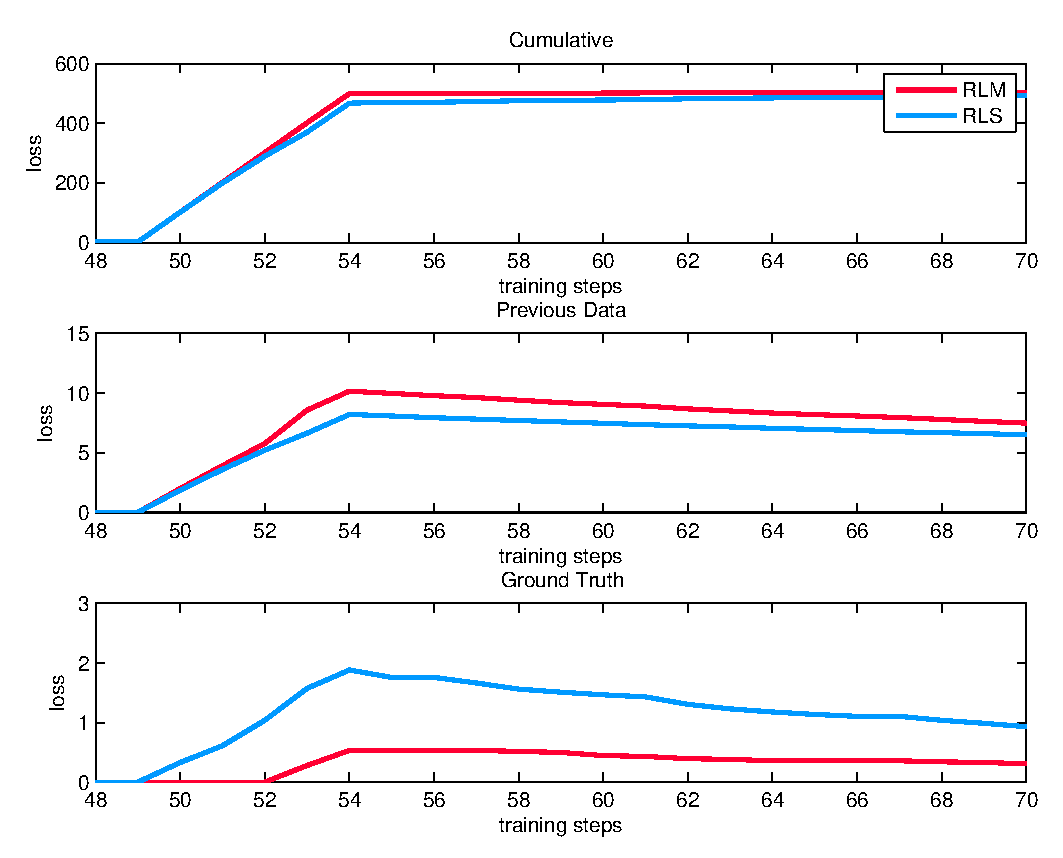
\includegraphics[width=\textwidth]{./images/copyofstats/impuls6row4_perf_100.eps}
                \caption{}
                \label{fig:perf:improw:perf}
        \end{subfigure}
        \\
        \caption{Approximation und Performance-Ergebnisse bei polynomiellem Approximator 4. Grades auf impulsversetzten Daten in Reihe.}
        \label{fig:perf:improw}
\end{figure}
In diesem Szenario wird auf weitere Grenzen des RLM mit impulsversetzten Daten eingegangen. Dazu wird $N = 6$ gesetzt um dessen Einfluss auf diese Situation zu zeigen.
An Abb. (\ref{fig:perf:improw:perf}) ist zu erkennen, dass mit Beginn der Impulsreihe der RLS einen ansteigenden Previous-Data Loss aufweist. Der RLM hingegen zeigt hier keinen Anstieg. Ferner ist zu beobachten, dass zu Zeitpunkt 53, also beim 4. Lerndatum auch beim RLM ein Anstieg zu verzeichnen ist. Grund hierfür ist das klein gewählte $N$, welches dazu führt, dass in Reihe vorkommende große Fehler nun vom Median auch beachtet werden, da diese 4 von 6 Elementen in ihm ausmachen.
In der Approximation in Abb. (\ref{fig:perf:improw:approx}) ist daher auch zu erkennen, dass der RLS auf Höhe aller Impulse nach unten gezogen ist, der RLM hingegen nur bei den letzten Impulsen eine negative Abweichung aufweist.
Durch die Wahl eines größeren $N$, kann diesem Effekt entgegengewirkt werden.

\subsection{Bewertung}
\label{sec:perf:bewertung}
In diesem Abschnitt werden die Inhalte der einzelnen Szenarien zusammengefasst und dazu Stellung genommen. Außerdem wird ein weiteres robuste Lernverfahren kurz vorgestellt und mit dem RLM in Beziehung gesetzt.

Für die Bewertung des RLM gilt die Annahme für potenzielle Szenarien, dass Ausreißer/Impulse in den Lerndaten \emph{nicht} in die Approximation miteinbezogen werden sollen. Sofern diese Annahme nicht gelten soll, ist von der Verwendung des RLM abzuraten.

Insgesamt lässt sich sagen, dass der RLM es schafft einzelne Impulse in Daten zu erkennen und diese nicht in sein Parameter- und Adaptionsupdate miteinzubeziehen. Genau diese Eigenschaft ist in vielen Fällen jedoch problematisch. Denn vorallem in der Anfangsphase werden hohe Fehlerwerte, welche zu Beginn als normal zu betrachten sind, als Ausreißer interpretiert. Dadurch verzögert sich die Annäherung an die Zielfunktion.
Im Gegensatz dazu werden Impulse, welche zu Beginn auftreten auch korrekt ignoriert.
In den hier vorgestellten Szenarien spielen sich die Unterschiede in der Approximationsgeschwindigkeit zwischen RLM und RLS  in einem Rahmen von ca. 10 Lerndaten ab. Sofern auf die Impulserkennung in der initialen Phase nicht verzichtet werden kann, muss das verzögerte Einpendeln in Kauf genommen werden.
Wird an Stelle eines globalen, ein lokaler Approximator verwendet, so könnte die Adaption gerade in der Anfangsphase schneller laufen. Dazu muss die Standardabweichung in Abhängigkeit zu der Differenz zwischen der Nulllinie des Approximators und den präsentierten Daten gewählt werden.
Wie in den 4 Graphen in Abb. (\ref{fig:perf:ausdruck:approx}) erkennbar ist, verhält sich die Annäherung des RLM im Laufe des Lernprozesses unruhig. Damit ist gemeint, dass die Kurven zu zwei aufeinanderfolgenden Zeitpunkten stark voneinander abweichen können.
Bei lokalen Approximatoren wird dieses Verhalten abgeschwächt, da die Funktionsabschnitte beispielsweise nicht ins Unendliche wachsen können.

Generell ist die Performance des RLM am besten gegenüber dem RLS, wenn die Daten Ausreißer enthalten, welche nicht in die Approximation miteinbezogen werden sollen. In den anderen vorgestellten Szenarien hat der RLM eine schlechtere bzw. gleiche Performance wie der RLS aufgezeigt.
Bei zeitvarianten Zielfunktionen ist von der Verwendung des RLM eher abzuraten, da dort die Wahrscheinlichkeit einer Fehlinterpretation hoher Fehler groß ist.

\subsubsection{Proposed Robust RLS (PRRLS)}
\label{sec:perf:bewertung:prrls}
Ein anderer Ansatz für ein robustes Lernverfahren wird mit dem \emph{Proposed Robust RLS (PRRLS)} \cite{bhotto2011robust} verfolgt. Kern des Verfahrens ist die $L_1$-Norm des Kreuzkorrelationsvektors einzudämmen. Ein hoher Fehler $e_n$ führt zu einem Anstieg der $L_1$-Norm von $\|P_n - \lambda P_{n-1}\|$, was dem Algorithmus als Indikator dient Ausreißer zu kennen. Wie bereits erwähnt wird nun versucht die $L_1$-Norm einzudämmen indem diese einen gewissen Upper Bound $\gamma_n$ nicht überschreiten darf.
\begin{align}
  \|P_n - \lambda P_{n-1}\| \leq \gamma_n = \left|\frac{d_n}{e_n}\right| \nonumber
\end{align}
Bewerkstelligt wird diese Bedingung mittels einer Variablen
\begin{align}
  \delta_n = \text{min}\left\{1,\frac{1}{\|x_n e_n\|_1}\right\} \nonumber
\end{align}
welche im Update von $S_n$ und $\alpha_n$ vorkommt
\begin{align}
  \label{eq:perf:bewertung:s}
  S_n &= \frac{1}{\lambda}\left( S_{n-1} - \frac{1}{\frac{\lambda}{\delta_n} + x_n^TS_{n-1}x_n} S_{n-1}x_n x_n^TS_{n-1} \right)\\
  \label{eq:perf:bewertung:alpha}
  \alpha_n &= \alpha_{n-1} + \frac{1}{\frac{\lambda}{\delta_n} + x_n^TS_{n-1}x_n} S_{n-1}x_n e_n
\end{align}
Wenn der Fehler klein ist, dann gilt $\frac{1}{\|x_n e_n\|_1} \geq 1$ also $\delta_n=1$, was dazu führt, dass der PRRLS sich genau wie der RLS verhält.
Sollte ein impulsversetztes Datum auftreten, gilt $\frac{1}{\|x_n e_n\|} < 1$ also $\delta_n=\frac{1}{\|x_n e_n\|_1}$ was zu einer Hemmung des Parameterupdates führt (siehe Bruch in Gleichungen (\ref{eq:perf:bewertung:s}) und (\ref{eq:perf:bewertung:alpha})).

Während der RLM die letzten $N$ Fehler als Grundlage für die Impuls-Interpretation verwendet, findet beim PRRLS ein Vergleich seiner aktuellen Approximation mit dem aktuellen Fehler statt. 
Dies hat zur Folge, dass der RLM bei vielen großen Fehlern seine Grenzen dementsprechend anpasst und diese großen Fehler approximiert. Der PRRLS macht die Toleranz nicht anhand der letzten $N$ Fehler fest.
Im Szenario aus Abschnitt (\ref{sec:perf:impulse:reihe}) hat der PRRLS einen Vorteil gegenüber dem RLM, da beim PRRLS die Länge der Impulsreihe keine Rolle spielt. Sobald beim RLM hingegen $\left\lceil \frac{N}{2} \right\rceil$ Impulse präsent waren, versucht er ab dem nächsten Impuls diese auch abzubilden.

Die Verwendung des PRRLS sollte also in Betracht gezogen werden, wenn nicht absehbar ist wie lange eventuell vorkommende Impulsreihen sind. Ist die Länge bekannt kann durch Parametrisierung eines entsprechendem $N$ dem im RLM vorgebeugt werden.

\section{Zusammenfassung}
\label{sec:zusammenfassung}
Im Rahmen dieser Ausarbeitung wurde der Recursive Least M-Estimate Algorithmus, ein RLS ähnliches Lernverfahren vorgestellt. Der RLM hat als Ziel hohe Fehlerwerte aus seinem Parameter- und Adaptionsupdate herauszuhalten und stellt somit ein robustes Lernverfahren dar.
Durch Messungen in verschiedenen Szenarien wurde seine Performance mit der des RLS verglichen und abschließend bewertet und dessen Grenzen und Besonderheiten aufgeführt.
\newpage
% Bibliography
\bibliographystyle{ieeetr}
\bibliography{rlm}

\newpage
\appendix
\section{Weitere Graphen/Abbildungen}
\subsection{Graphen zur Ausdrucksstärke}
\label{apx:ausdruck}
\begin{figure}[H]
        \centering
        \begin{subfigure}[b]{0.4\textwidth}
                \centering
                \includegraphics[width=\textwidth]{./images/copyofstats/ausdruck1_approx_100poly.eps}
                \caption{}
                \label{fig:apx:ausdruck:ausdruck11}
        \end{subfigure}
        \begin{subfigure}[b]{0.4\textwidth}
                \centering
                \includegraphics[width=\textwidth]{./images/copyofstats/ausdruck1_perf_100poly.eps}
                \caption{}
                \label{fig:apx:ausdruck:perf11}
        \end{subfigure}
        \\
        \caption{Approximation und Performance-Ergebnisse bei linearem Approximator auf polynomiellen GroundTruth-Daten.}
        \label{fig:apx:ausdruck1}
\end{figure}

\subsection{Graphen zu Trajektorieneffekten}
\label{apx:trajektorien}
\begin{figure}[H]
        \centering
        \begin{subfigure}[b]{0.4\textwidth}
                \centering
                \includegraphics[width=\textwidth]{./images/copyofstats/trajektorien1_approx_100.eps}
                \caption{}
                \label{fig:apx:trajektorien1:approx}
        \end{subfigure}
        \begin{subfigure}[b]{0.4\textwidth}
                \centering
                \includegraphics[width=\textwidth]{./images/copyofstats/trajektorien1_perf_100.eps}
                \caption{}
                \label{fig:apx:trajektorien1:perf}
        \end{subfigure}
        \\
        \caption{Approximation und Performance-Ergebnisse bei linearem Approximator auf linearen GroundTruth-Daten mit Trajektorieneffekten.}
        \label{fig:apx:trajektorien1}
\end{figure}
\begin{figure}[H]
        \centering
        \begin{subfigure}[b]{0.4\textwidth}
                \centering
                \includegraphics[width=\textwidth]{./images/copyofstats/trajektorien1_approx_100.eps}
                \caption{}
                \label{fig:apx:trajektorien3:approx}
        \end{subfigure}
        \begin{subfigure}[b]{0.4\textwidth}
                \centering
                \includegraphics[width=\textwidth]{./images/copyofstats/trajektorien1_perf_100.eps}
                \caption{}
                \label{fig:apx:trajektorien3:perf}
        \end{subfigure}
        \\
        \caption{Approximation und Performance-Ergebnisse bei polynomiellem Approximator 3. Grades auf linearen GroundTruth-Daten mit Trajektorieneffekten.}
        \label{fig:apx:trajektorien3}
\end{figure}

\subsection{Graphen zu nichtlinearen Zielfunktionen}
\label{apx:nichtlinear}
\begin{figure}[H]
        \centering
        \begin{subfigure}[b]{0.3\textwidth}
                \centering
                \includegraphics[width=\textwidth]{./images/copyofstats/nonlin3_approx_13.eps}
                \caption{Approx. nach 13 Daten.}
                \label{fig:apx:nichtlinear:approx13}
        \end{subfigure}
        \begin{subfigure}[b]{0.3\textwidth}
                \centering
                \includegraphics[width=\textwidth]{./images/copyofstats/nonlin3_approx_100.eps}
                \caption{Approx. nach 100 Daten.}
                \label{fig:apx:nichtlinear:approx100}
        \end{subfigure}
        \begin{subfigure}[b]{0.3\textwidth}
                \centering
                \includegraphics[width=\textwidth]{./images/copyofstats/nonlin3_perf_100.eps}
                \caption{Perf. nach 100 Daten.}
                \label{fig:apx:nichtlinear:perf100}
        \end{subfigure}
        \\
        \caption{Approximation und Performance-Ergebnisse bei polynomiellen Approximator 3. Grades auf nichtlinearen GroundTruth-Daten.}
        \label{fig:apx:nichtlinear}
\end{figure}

\section{Matlab Code}
\label{apx:matlab}
\subsection{Initialisierungsmethode des RLM}
\label{apx:matlab:init}
\lstinputlisting[language=Matlab, deletekeywords={eps}, morekeywords={...,isfield}]{icl_initILS_RLM.m}

\subsection{Lernmethode des RLM}
\label{apx:matlab:learn}
\lstinputlisting[language=Matlab, deletekeywords={eps}, morekeywords={...,isfield},]{icl_learn_RLM.m}

\subsection{Impulsgenerierung}
\label{apx:matlab:imp}
\lstinputlisting[language=Matlab, deletekeywords={eps}, morekeywords={...,isfield}]{icl_genImpulses.m}

\end{document}